\section{Textual use case format and editor}

Textual use case format allows to write use cases using plain-text. The format is proposed for rapid writing of the use cases and its subsequent import into Reprotool project.

Structure of the format as well as developed textual editor is described in
the following subsections.

\subsection{Structure of the textual use case}

Grammar of the textual use case allows to enter \textit{Use case name}, \textit{Description}, \textit{Primary actor} of the use case, \textit{Preceding use cases}, \textit{Main scenario} of the use case, it's \textit{Extensions} and \textit{Variations} in this particular order.

\begin{figure}[ht]
  \centering
  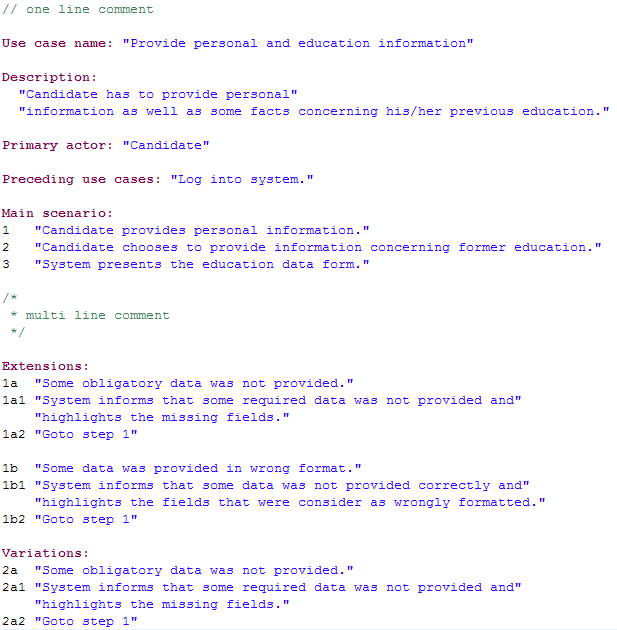
\includegraphics[height=400pt]{images/txtuc-editor/filledTxtuc}
  \caption{Textual use case example}
  \label{fig:filledTxtuc}
\end{figure}

Use of the \textit{Preceding use cases}, \textit{Extensions} and \textit{Variations} is optional, all other parts are mandatory.

Values used in parts (value of the \textit{Use case name}, step of the \textit{Main scenario} etc) are enclosed in double quotes and use same escaping rules as strings in Java programming language.

Description and use case steps (and conditions preceeding steps in Extensions/Variations) may be split into multiple consecutive strings (each may be placed on it's own line).

Format allows to insert comments. Their format is same as in Java - one line comments are prefixed with "\verb|//|" and multiline are enclosed between "\verb|/*|" and "\verb|*/|" character sequences.

Numbers of the use case steps start from one and must form consecutive sequence. Similar rule applies for use case steps in extensions and variations scenario with addition that their number must be prefixed with label of the corresponding condition (e.g. "\verb|5a1|"). Condition label has to reference existing use case step and last  letters used in labels of the conditions must also form consecutive sequence (for example - next condition after \verb|5a| must be followed by \verb|5b|).

Example of the textual use case is shown in Figure~\ref{fig:filledTxtuc}


\subsection{Textual use case editor}

To create new textual use case select \verb|"File" -> "New" -> "Textual use case"| and fill file name (e.g. "\verb|register|"). Empty use case from predefined template should open as seen in Figure~\ref{fig:emptyTxtuc}.

\begin{figure}[ht]
  \centering
  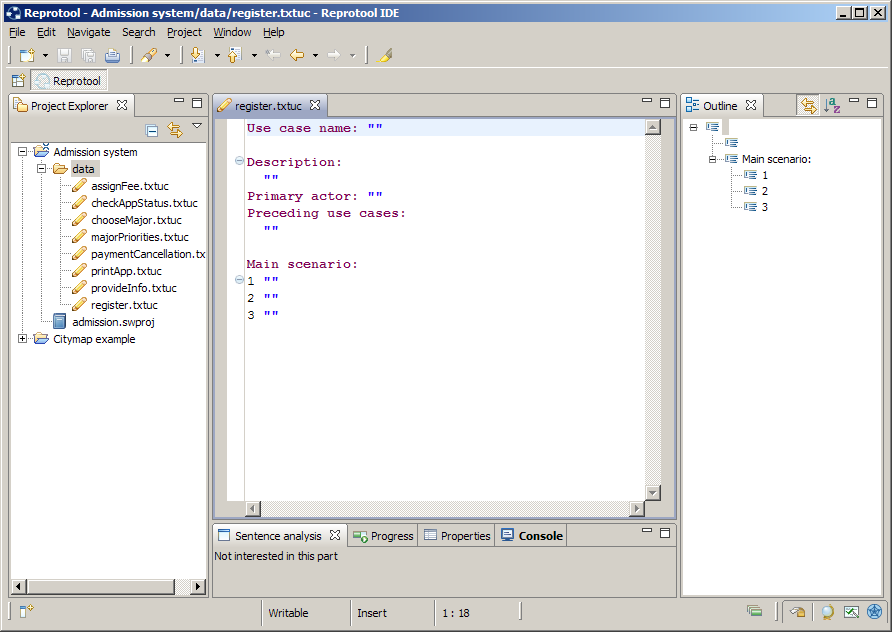
\includegraphics[height=280pt]{images/txtuc-editor/emptyTxtuc}
  \caption{Empty textual use case}
  \label{fig:emptyTxtuc}
\end{figure}

Use \verb|ctrl + space| during use case writing to open content assist (see Figure~\ref{fig:contentAssist}). Violations against use case step format are indicated with error markers as shown on Figure~\ref{fig:wrongLabel}.
Outline page shows structure of the textual use case. Selection of the item in content outline affects selection in the editor and vice-versa.

\begin{figure}[ht]
  \centering
  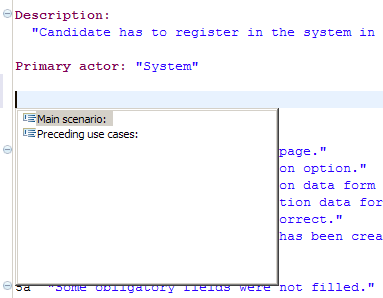
\includegraphics[width=8cm]{images/txtuc-editor/contentAssist}
  \caption{Content assist}
  \label{fig:contentAssist}
\end{figure}

\begin{figure}[ht]
  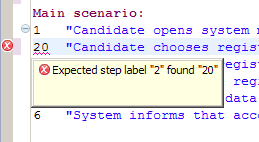
\includegraphics[width=6cm]{images/txtuc-editor/wrongLabel}
  \caption{Error marker for wrong label}
  \label{fig:wrongLabel}
\end{figure}




